% Toolbar icon: fieldHessian — the second derivative of a field, drawn as a
% 3x3 matrix of dots inside brackets: the Hessian IS a 3x3 matrix, and the
% result is stored as its 9 flattened components. Deliberately distinct from
% `fieldCalc`'s calculator grid (2x3 dots in a framed button with a display
% bar) — brackets, not a frame, and three rows, not two.
\documentclass[tikz,border=2mm]{standalone}
\usetikzlibrary{arrows.meta,calc,shapes.geometric}
\begin{document}
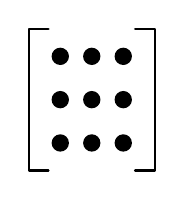
\begin{tikzpicture}[line width=1.3pt, line cap=round, line join=round, x=1mm,y=1mm]
  % Matrix brackets.
  \draw[thick] (-5.5,-9) -- (-8,-9) -- (-8,9) -- (-5.5,9);
  \draw[thick] (5.5,-9) -- (8,-9) -- (8,9) -- (5.5,9);
  % 3x3 of entries.
  \foreach \x in {-4,0,4} {
    \foreach \y in {-5.5,0,5.5} {
      \fill (\x,\y) circle (1.1);
    }
  }
\end{tikzpicture}
\end{document}
